\documentclass{article}

\usepackage{graphicx}
\usepackage{multicol}
\usepackage[center]{titlesec}
\usepackage{geometry}
\usepackage{mathtools}



%
%\setlength{\columnseprule}{0.4pt}
%\setlength{\footskip}{20pt}
\usepackage{fancyhdr}
\fancyhf{}
\fancyhead[C]{Joe Brew $\bullet$ FDOH-Alachua $\bullet$ Ben Brew}
\fancyfoot[C]{  $\bullet$ Mosquito Surveillance Report \bullet$  }
\renewcommand\headrulewidth{1pt}
\renewcommand\footrulewidth{1pt}
\pagestyle{fancy}

%

\setlength{\columnsep}{1.5cm}
%\setlength{\columnseprule}{0.4pt}

%\MakeOuterQuote{"}



\graphicspath{ {E:/fdoh/public/mosquito/reports/2014-08-21} }

%the next two lines adjust the third, centered section of the exec sum
\def\changemargin#1#2{\list{}{\rightmargin#2\leftmargin#1}\item[]}
\let\endchangemargin=\endlist 

\usepackage{Sweave}
\begin{document}
\Sconcordance{concordance:mosquitoReport.tex:mosquitoReport.Rnw:%
1 36 1 1 0 17 1 1 20 82 1 1 88 1 3 12 1 1 27 1 2 19 1 1 24 1 2 12 1 1 %
30 1 2 14 1 1 98 1 2 10 1 1 13 1 2 10 1 1 22 1 4 1 1 1 22 1 3 39 1}


\title{\textbf{Mosquito Surveillance Report}}
\author{Joe Brew and Ben Brew}


\maketitle
\tableofcontents

\vspace{40mm}

\begin{center}

\includegraphics[width=2cm]{doh}
\end{center}





\newgeometry{margin=5cm}
\fancyhfoffset[E,O]{0pt}


\vspace*{30mm}
%------------------------------------------
\section*{Executive Summary}
\addcontentsline{toc}{section}{Executive Summary}
%------------------------------------------
\hrulefill




\begin{multicols}{2} 
\setkeys{Gin}{width=0.49\textwidth}


%------------------------------------------
\subsection*{Most Recent Collection}
%------------------------------------------

As predicted, mosquito numbers remained largely steady over recent weeks, peaking slightly at the most recent trap collection (August 05, 2014) (242 mosquitoes per trap).  

\vfill
\columnbreak



%------------------------------------------
\subsection*{Forecast}
%------------------------------------------

We forecast that mosquito levels will remain in the moderate range over the next week (approximately 150 mosquitoes per trap), with a 95\% confidence interval of 0 to 302 per trap.  



\end{multicols}
\setkeys{Gin}{width=1\textwidth}

\vspace{2mm}
%------------------------------------------
\subsection*{Predictive Model Validation}
%------------------------------------------


\begin{changemargin}{1.5cm}{1.5cm} 

At 242 specimens per trap, the most recent collection was significantly higher than our prediction of 86, but remained (barely) within the 90\% confidence range of 0-242.  

\end{changemargin}

\hrulefill


\newgeometry{margin=2.5cm}
\fancyhfoffset[E,O]{0pt}
%------------------------------------------
%\section*{Visual Overview}
%\addcontentsline{toc}{section}{Visual Overview}
%------------------------------------------


%------------------------------------------
\section*{Visual Overview}
\addcontentsline{toc}{section}{Visual Overview}
%------------------------------------------
\hrulefill

\begin{multicols}{2} 
\setkeys{Gin}{width=0.49\textwidth}



%------------------------------------------
\subsection*{Time}
\addcontentsline{toc}{subsection}{Time}
%------------------------------------------
The current mosquito population is lower than usual for this time of year.
\begin{center}
%\begin{figure}
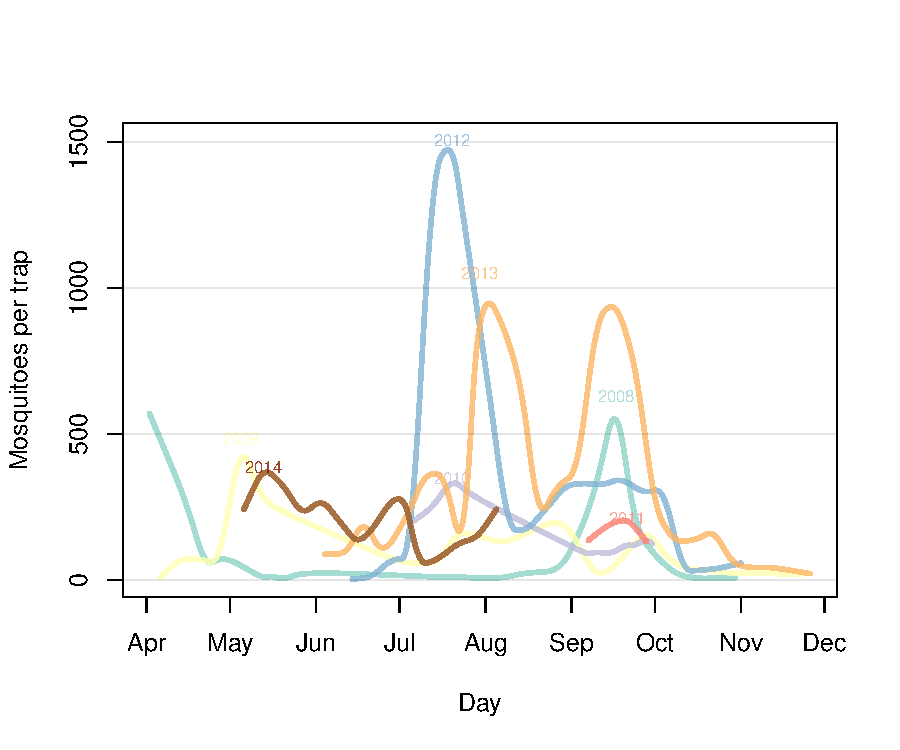
\includegraphics{mosquitoReport-002}
%\caption{Yearly comparison}
%\end{figure}
\end{center}


\vfill
\columnbreak
%------------------------------------------
\subsection*{Space}
\addcontentsline{toc}{subsection}{Space}
%------------------------------------------
Mosquitoes were largely scattered throughout the county.

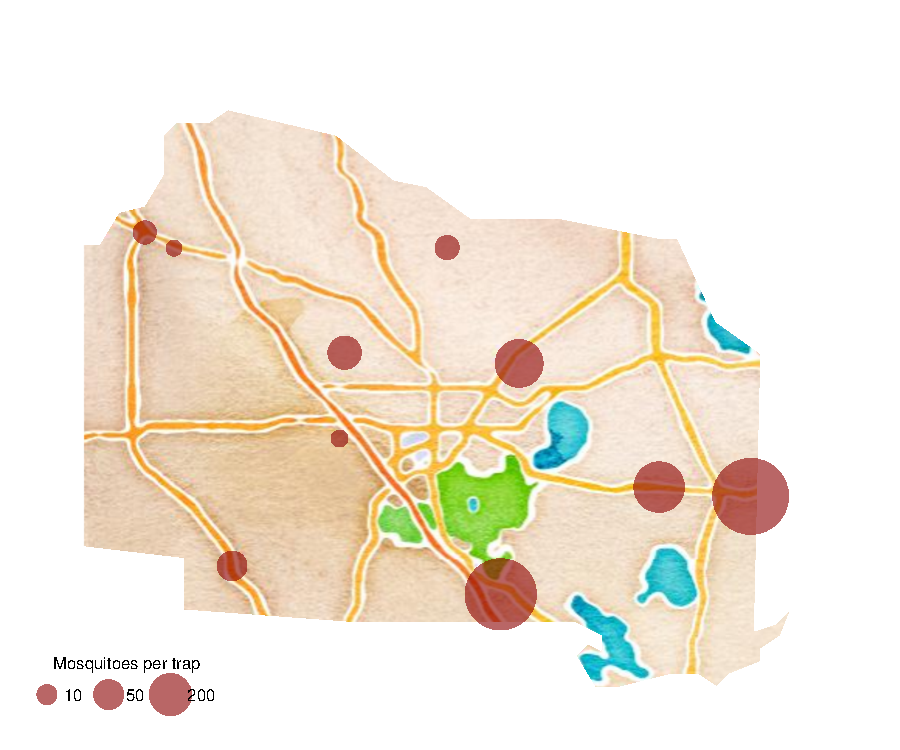
\includegraphics{mosquitoReport-003}

\end{multicols}
\setkeys{Gin}{width=1\textwidth}


%\hrulefill
\vspace{10mm}

\begin{multicols}{2} 
\setkeys{Gin}{width=0.49\textwidth}


\vfill
\columnbreak
%------------------------------------------
\subsection*{Normality}
\addcontentsline{toc}{subsection}{Normality}
%------------------------------------------
The most recent collection was at levels equivalent to approximately the 72nd percentile of historical (2008-13) levels.

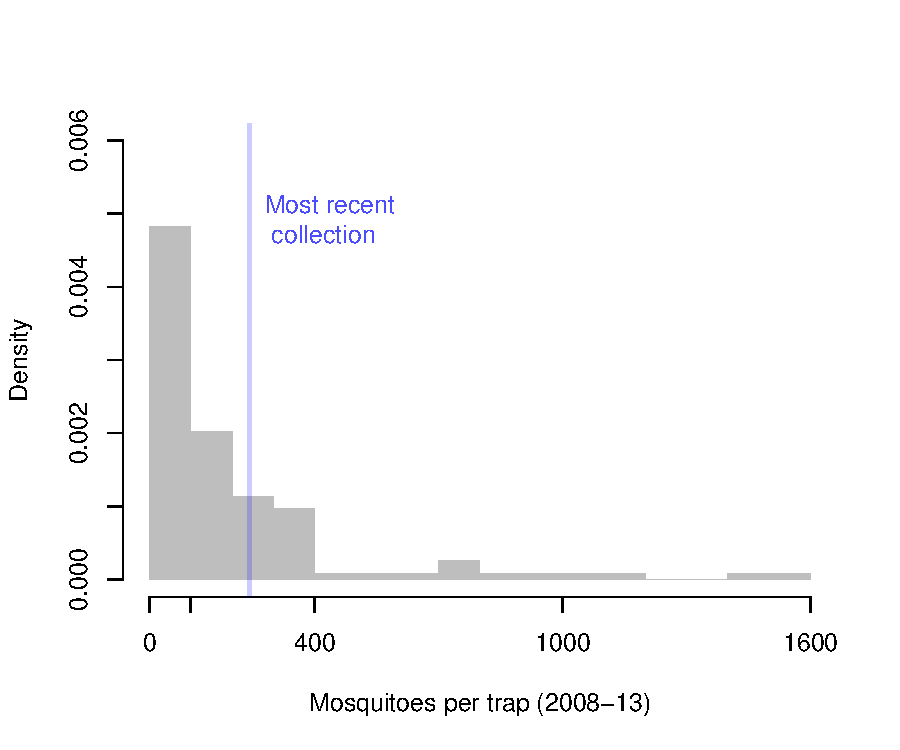
\includegraphics{mosquitoReport-004}

\vfill
\columnbreak



%------------------------------------------
\subsection*{Disease Vectors}
\addcontentsline{toc}{subsection}{Disease Vectors}
%------------------------------------------

Mosquitoes capable of carrying WNV have seen increases over the last few weeks, particularly in the southeastern part of the county.

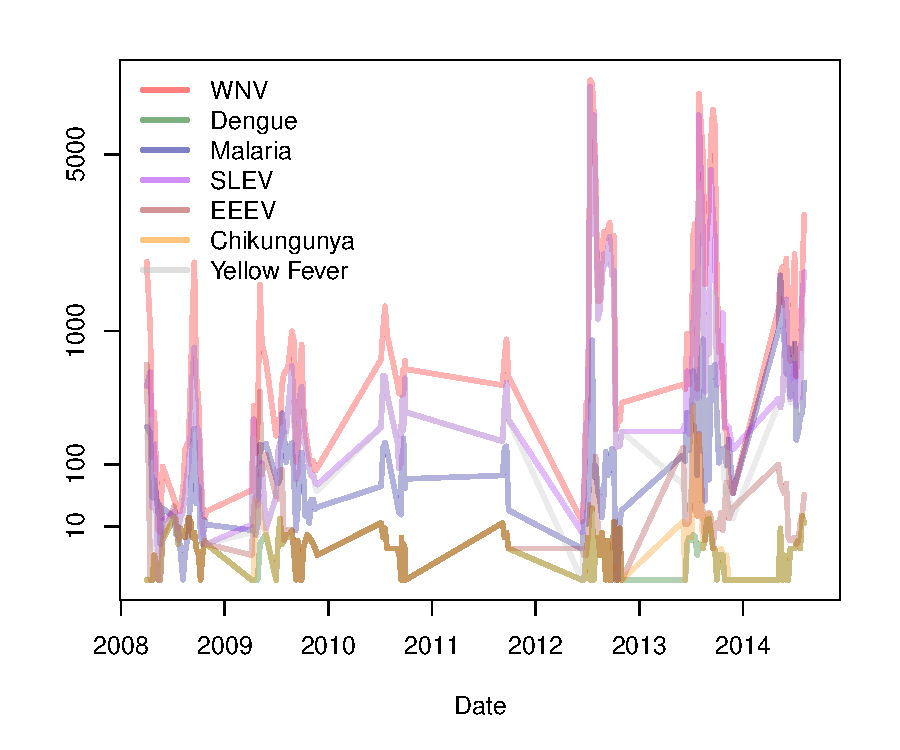
\includegraphics{mosquitoReport-005}

\vfill
\newpage
\end{multicols}
\setkeys{Gin}{width=1\textwidth}

%------------------------------------------
\section*{Forecast}
\addcontentsline{toc}{section}{Forecast}
%------------------------------------------
\hrulefill
\vspace{5mm}

\noindent We use recursive, quadratic linear regression modelling to forecast the average number of mosquitoes per trap up to 15 days in advance.\footnote{We are actively experimenting with non-parametric approaches to improve modelling accuracy, and expect to have a modified KNN model with better results by late August.}  

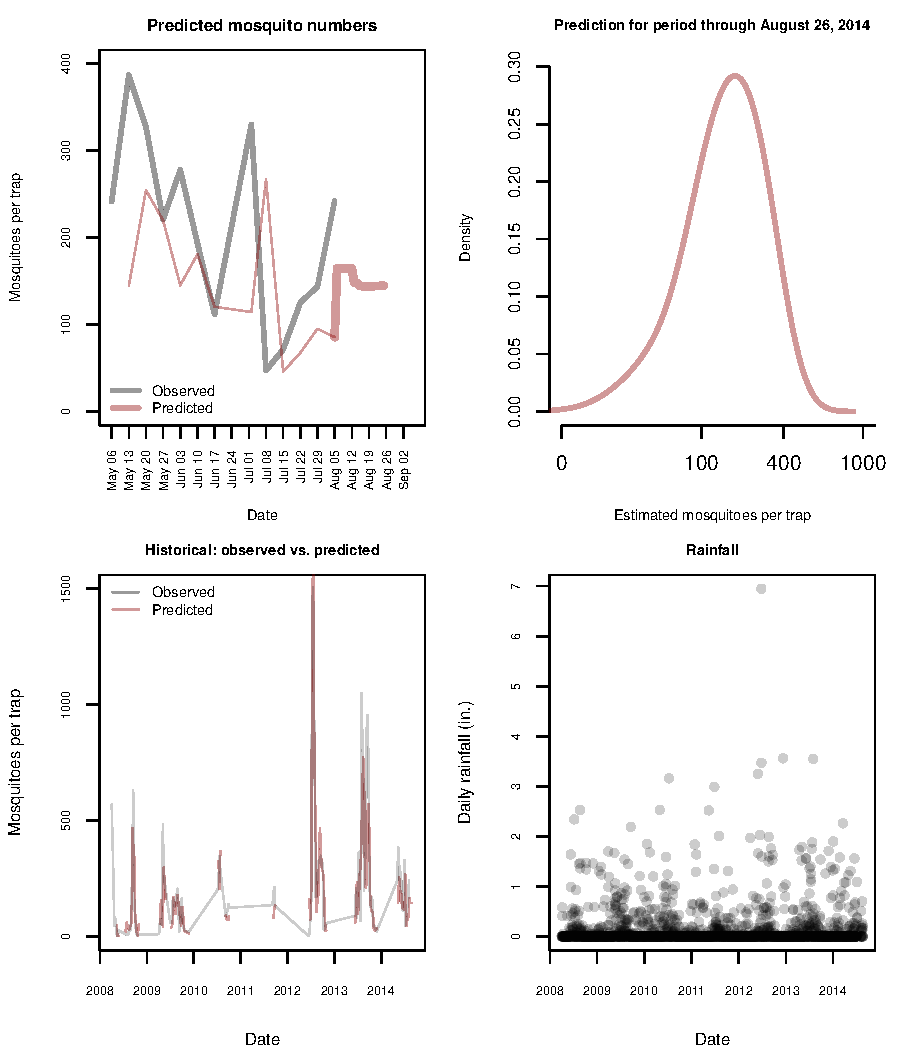
\includegraphics{mosquitoReport-006}


\newpage

%------------------------------------------
\section*{Vectors of Disease by Location}
\addcontentsline{toc}{section}{Vectors of Disease by Location}
%------------------------------------------
\hrulefill
\vspace{5mm}

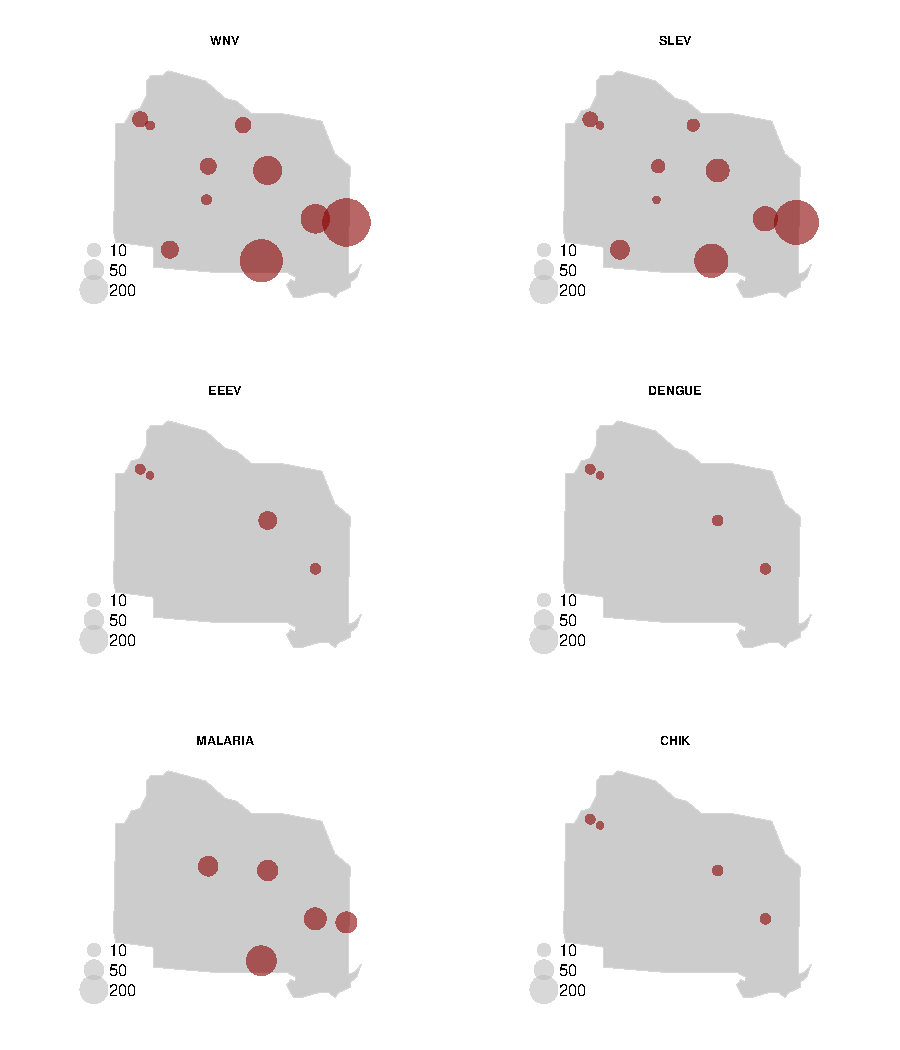
\includegraphics{mosquitoReport-007}


%------------------------------------------
\section*{Mosquito Types}
\addcontentsline{toc}{section}{Mosquito Types}
%------------------------------------------
\hrulefill
\vspace{5mm}

Uranotanneaia sapphirina saw large increases in population in recent weeks. 


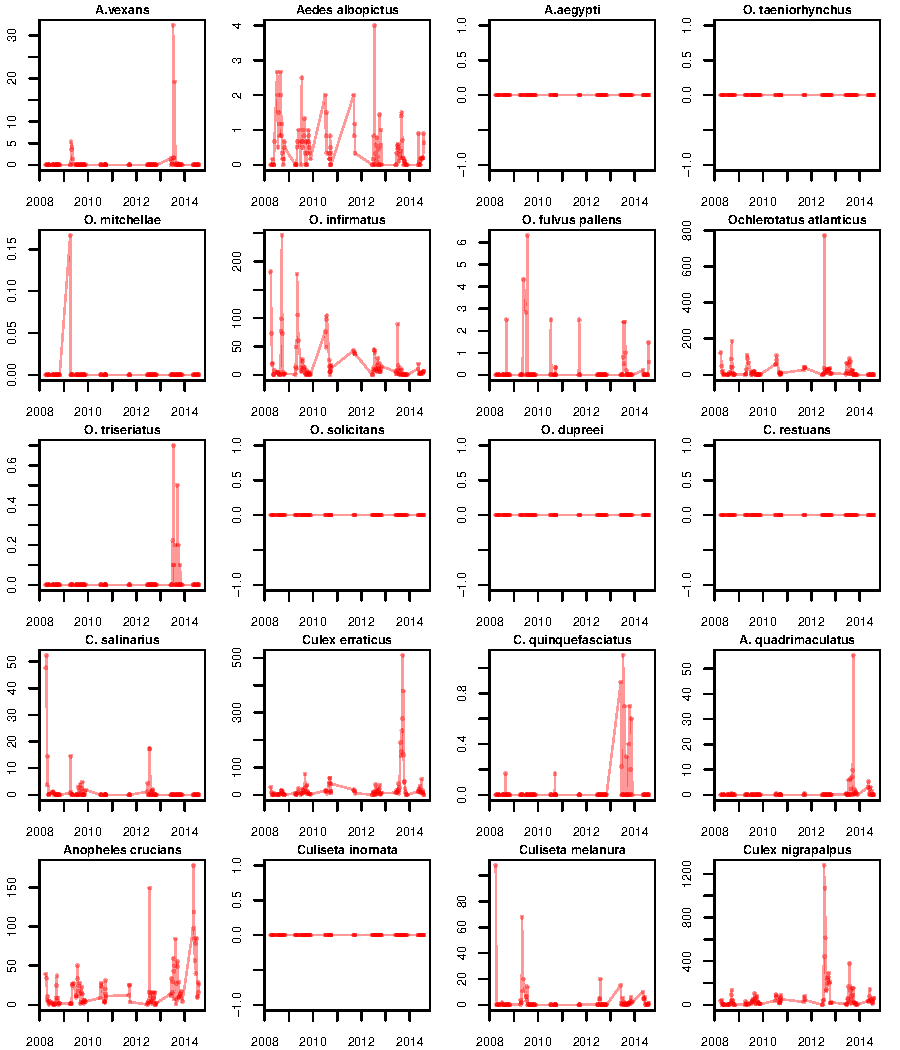
\includegraphics{mosquitoReport-008}


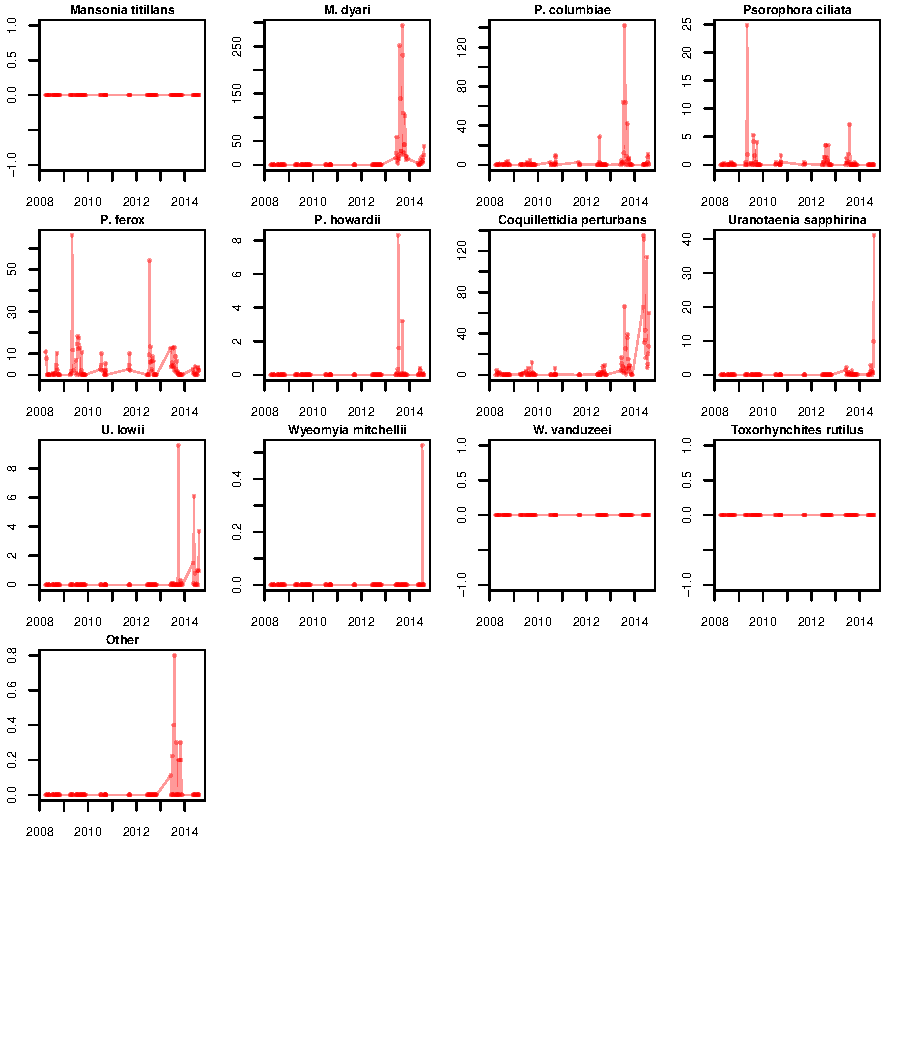
\includegraphics{mosquitoReport-009}




% \begin{multicols}{2} 
% \setkeys{Gin}{width=0.49\textwidth}

% \end{multicols}
% \setkeys{Gin}{width=1\textwidth}
% \end{adjustwidth*}





\newpage
%------------------------------------------
\section*{Details of Predictive Model}
\addcontentsline{toc}{section}{Details of Predictive Model}
%------------------------------------------
\hrulefill
\vspace{5mm}

Historically, the model has performed well, correctly predicting the late summer spikes in 2012 and 2013.  Given the preference for accuracy at high numbers, the model intentionally includes outlying high observations, thereby weighting them. \\

Having simulated more than 65,000 unique models, our best fit equation (using the sum of least squares approach) was: 

\begin{center} 
$\hat{Y} = \beta_0+ \beta_1^2 (5.6508)$ + \beta_2 (0.5938)$ 
\end{center}

\noindent where $\hat{Y}$ is the estimated mean number of mosquitoes per trap, $\beta_0$ is set to 0, $\beta_1$ is the cumulative rainfall in the period 15 to 29 days prior to the date of prediction and $\beta_2$ is the mean number of mosquitoes per trap in the most recent prior trap collection.  \\

Though an original model relied only on rainfall, incorporating the most recent trap predicition saw our R-squared improve from 0.52 to 0.82.  This means that we can now explain over 80\% of the variance in mosquito populations up to 15 days ahead of time.  





\end{document}
